\بابء{علامات}

اس کتاب میں بین الاقوامی نظامِ اکائی \تحریر{SI} استعمال کیا گیا ہے۔یوں میٹر، کلو گرام اور سیکنڈ کے علاوہ وولٹ، ایمپیئر، اوہم اور واٹ کو جوں کا توں استعمال کیا جائے گا۔

برقی دباو، برقی رو اور ان کی مخصوص خصلتیں اجاگر کرانے کی خاطر مختلف علامتیں استعمال کی جاتی ہیں۔ان علامتوں کو، جن سے بخوبی واقف ہونا ضروری ہے، یہاں پیش کرتے ہیں۔

\begin{description}
\item
[\عددی{V_{DD},V_{CC},V_{EE},V_{BB}}]  پیدا کار یک سمتی برقی دباو
\item
[\عددی{V_{BE}, V_{CE},I_D, I_C}] یک سمتی برقی دباو اور برقی رو  (اشارہ موجود یا عدم موجود)
\item
[\عددی{V_{CEQ},I_{CQ}}]  نقطہ کارکردگی پر یک سمتی برقی دباو اور برقی رو (اشارہ عدم موجود)
\item
[\عددی{v_d , v_{be},i_d,i_c,i_e}] بدلتا اشارہ (اوسط قیمت صفر)
\item
[\عددی{I_d, I_c,I_e,I_b} ]  سائن نما برقی رو کی موثر قیمت (rms)
\item
[\عددی{V_{dm},V_{cem},I_{dm},I_{cm}} ]  اشارے کی چوٹی
\item
[\عددی{v_{D},v_{BE},v_{CE},v_{BC}} ] لمحاتی برقی دباو
\item
[\عددی{i_D,i_C,i_E,i_B} ] لمحاتی برقی رو
\end{description}

\FloatBarrier

ان کی مزید وضاحت شکل \حوالہ{شکل_سائن_نما_اشارے_کے_جزو}  اور شکل \حوالہ{شکل_غیر_سائن_نما_اشارے_کے_جزو} میں کی گئی ہے۔

\begin{figure}
\centering
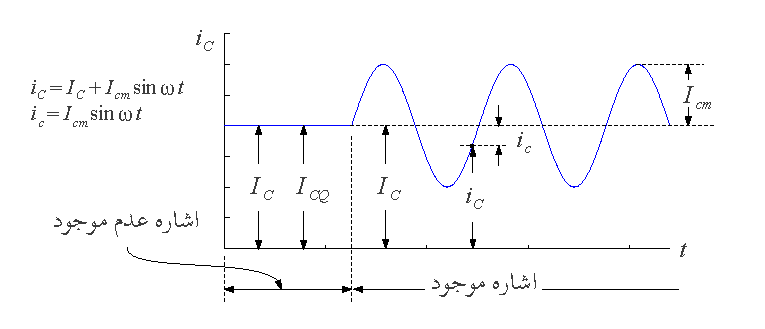
\includegraphics[scale=0.90]{definingSinusoidalWaveParameters}
\caption{سائن نما اشارہ}
\label{شکل_سائن_نما_اشارے_کے_جزو}
\end{figure}

\begin{figure}
\centering
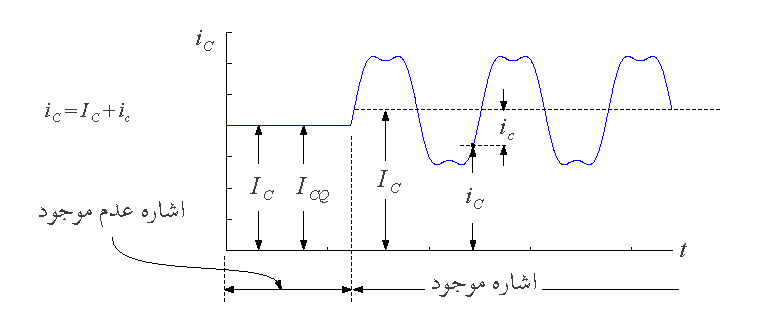
\includegraphics[scale=0.90]{definingNonSinusoidalWaveParameters}
\caption{غیر سائن نما اشارہ}
\label{شکل_غیر_سائن_نما_اشارے_کے_جزو}
\end{figure}

\FloatBarrier



\begin{tabular}{r l}
\hline
\multicolumn{2}{c}{اصطلاحات} \\
\hline
برقی دباو & \تحریر{voltage}\\
برقی رو & \تحریر{current} \\
برقی مزاحمت & \تحریر{resistance} \\
کپیسٹر & \تحریر{capacitor} \\
امالہ & \تحریر{inductor} \\
برقی رکاوٹ & \تحریر{impedance} \\
پیدا کار برقی دباو & \تحریر{voltage source}\\
پیدا کار برقی رو & \تحریر{current source} \\
تابع پیدا کار برقی دباو & \تحریر{dependent voltage source} \\
آزاد پیدا کار برقی دباو & \تحریر{independent voltage source} \\
حسابی ایمپلیفائر & \تحریر{OPAMP}\\
تفرقی جوڑا & \تحریر{difference pair} \\
اشارہ & \تحریر{signal} \\
پیدا کار اشارہ & \تحریر{signal generator}\\
تعدد & \تحریر{frequency} \\
دو جوڑ ٹرانزسٹر & \تحریر{BJT transistor}\\
ڈایوڈ  & \تحریر{diode}\\
ماسفیٹ & \تحریر{mosfet}\\
حیطہ سوار اشارہ & \تحریر{AM signal}
\end{tabular}
